\section{The Framework}
\label{sec:framework}
\begin{figure}[!h]
\begin{center}
\includegraphics[width=\columnwidth]{flowchat.eps}
\caption{Architecture of Wikification via Link Co-occurrence}
\label{fig:arch}
\end{center}
\end{figure}
%\KZ{Add another dash box in the figure 3 to mark out the preprocessing module.}

The framework of wikification via link co-occurrence
has a three-part architecture (See
\figref{fig:arch}): {\em preprocess of wiki data},
{\em co-occurrence matrix generation} and {\em document wikification}.
%\KZ{The first part does ...}
The first part collects a term-sense mapping from Wikipedia data and
parse Wikipedia articles to identify terms to be linked in the later parts.
The second part is an iterative process which, in each iteration, computes
the co-occurrence matrix from the current snapshot of the Wikipedia corpus,
and then use this matrix to disambiguate (i.e., add links to) noun phrases that
have not been linked yet in the corpus. The updated corpus will be used
in the next iteration. This part can be thought of as an off-line process.
The third part is an on-line process, which makes use of the final
co-occurrence matrix and converts a plain text to a text with links pointing
to relevant Wikipedia articles.

In the following sub-sections, we describe each of the three parts in
greater details.
%?g\begin{itemize}
%?g\item preprocessing on Wikipedia corpus and plain text
%?g%the generation of candidate sense lists for each surface form;
%?g%\item the parser that extract noun phrases from both plain text and partially
%?g%linked Wikipedia articles;
%?g\item the iterative enrichment of co-occurrence matrix and adding links
%?gto Wikipedia articles;
%?g\item wikification of a new document.
%?g\end{itemize}
%The architecture of our system is shown in
%The system consists of two main components:
%\emph{Co-occurrence matrix enrichment} and \emph{plain text Wikification}. We first generate candidate
%list which maps the surface form of a noun phrase to several Wikipedia entities. With the candidate list,
%we parse all of the Wikipedia articles. Then we iteratively build co-occurrence matrix, Wikify the parsed
%Wikipedia data, and again rebuild the co-occurrence matrix. After the enrichment process, we can use
%our learnt matrix to Wikify any plain text.

